% !TEX root = ../main.tex
\section{Introduction}
Logic circuits using DNA and RNA has many interesting applications in diagnostics and treatment. An example is cancer detection, where miRNA's can be used as biomarkers \cite{Peng2016}. These biomarkers can be used as inputs for logic circuits, which can be designed to activate FRET signals \cite{Seelig2006} or enzymes \cite{Engelen2016} when combinations of biomarkers are present or absent. For example, a circuit could be designed to activate when 2 unique miRNA's are present at the same time, or when a certain protein is present. This is represented schematically in figure \ref{example_circuit}.

\begin{figure}[h!]
\centering
\begin{circuitikz} \draw
  (0,3) node[and port] (and1) {}
  (2,2) node[or port] (or1) {}
  (and1.in 1) node [anchor=east] {miRNA 1}
  (and1.in 2) node [anchor=east] {miRNA 2}
  (and1.out) -| (or1.in 1)
  (or1.in 2) node [anchor=east] {Protein 1}
  (or1.out) node [anchor=west] {FRET or enzymatic activity}
;\end{circuitikz}
\label{example_circuit}
\caption{Example of logic circuit}
\end{figure}

The logic gates can be made using strand displacement \cite{Zhang2011}, where the outputs of one gate can be linked to the input of another by unique DNA or RNA sequences.

\begin{figure}[h!]
\centering
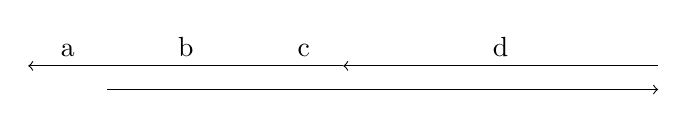
\begin{tikzpicture}
  \draw[<-](0,0.3) -- node[above] {a} (1,0.3);
  \draw(1,0.3) -- node[above] {b} (3,0.3);
  \draw(3,0.3) -- node[above] {c} (4,0.3);

  \draw[<-](4,0.3) -- node[above] {d} (8,0.3);

  \draw[->](1,0) -- (8,0);
\end{tikzpicture}
\label{}
\caption{Example of logic circuit}
\end{figure}
